\documentclass{beamer}
\mode<presentation>
\usepackage{amsmath}
\usepackage{amssymb}
 \usepackage{tkz-euclide}
%\usepackage{advdate}
\usepackage{adjustbox}
\usepackage{subcaption}
\usepackage{enumitem}
\usepackage{multicol}
\usepackage{listings}
\usepackage{graphicx}

 
\usepackage{url}
\hypersetup{
    colorlinks=true,
    linkcolor=blue,
    filecolor=magenta,      
    urlcolor=blue,
}
\def\UrlBreaks{\do\/\do-}
\usetheme{Boadilla}
\usepackage{gensymb}
\usepackage{tikz}
\usetikzlibrary{shapes.geometric,calc,angles,positioning,intersections,quotes,decorations,babel,patterns,fit}
\usepackage{tkz-euclide}
\usetkzobj{all}
\usecolortheme{lily}
\usepackage[utf8]{inputenc}
\usepackage[english]{babel}
\usepackage{hyperref}
\setbeamertemplate{footline}
{
  \leavevmode%
  \hbox{%
  \begin{beamercolorbox}[wd=\paperwidth,ht=2.25ex,dp=1ex,right]{author in head/foot}%
    \insertframenumber{} / \inserttotalframenumber\hspace*{2ex} 
  \end{beamercolorbox}}%
  \vskip0pt%
}
\setbeamertemplate{navigation symbols}{}
\providecommand{\nCr}[2]{\,^{#1}C_{#2}} % nCr
\providecommand{\nPr}[2]{\,^{#1}P_{#2}} % nPr
\providecommand{\mbf}{\mathbf}
\providecommand{\pr}[1]{\ensuremath{\Pr\left(#1\right)}}
\providecommand{\qfunc}[1]{\ensuremath{Q\left(#1\right)}}
\providecommand{\sbrak}[1]{\ensuremath{{}\left[#1\right]}}
\providecommand{\lsbrak}[1]{\ensuremath{{}\left[#1\right.}}
\providecommand{\rsbrak}[1]{\ensuremath{{}\left.#1\right]}}
\providecommand{\brak}[1]{\ensuremath{\left(#1\right)}}
\providecommand{\lbrak}[1]{\ensuremath{\left(#1\right.}}
\providecommand{\rbrak}[1]{\ensuremath{\left.#1\right)}}
\providecommand{\cbrak}[1]{\ensuremath{\left\{#1\right\}}}
\providecommand{\lcbrak}[1]{\ensuremath{\left\{#1\right.}}
\providecommand{\rcbrak}[1]{\ensuremath{\left.#1\right\}}}
\theoremstyle{remark}
\newtheorem{rem}{Remark}
\newcommand{\sgn}{\mathop{\mathrm{sgn}}}
\providecommand{\abs}[1]{\left\vert#1\right\vert}
\providecommand{\res}[1]{\Res\displaylimits_{#1}} 
\providecommand{\norm}[1]{\lVert#1\rVert}
\providecommand{\mtx}[1]{\mathbf{#1}}
\providecommand{\mean}[1]{E\left[ #1 \right]}
\providecommand{\fourier}{\overset{\mathcal{F}}{ \rightleftharpoons}}
%\providecommand{\hilbert}{\overset{\mathcal{H}}{ \rightleftharpoons}}
\providecommand{\system}{\overset{\mathcal{H}}{ \longleftrightarrow}}
	%\newcommand{\solution}[2]{\textbf{Solution:}{#1}}
%\newcommand{\solution}{\noindent \textbf{Solution: }}
\providecommand{\dec}[2]{\ensuremath{\overset{#1}{\underset{#2}{\gtrless}}}}
\newcommand{\myvec}[1]{\ensuremath{\begin{pmatrix}#1\end{pmatrix}}}
\let\vec\mathbf

\lstset{
%language=C,
frame=single, 
breaklines=true,
columns=fullflexible
}

\numberwithin{equation}{section}

\title{Algebraic approach to school Geometry}
\author{Priyanka}

\date{\today} 
\begin{document}

                                                                                                                                                                                                                                                                                                                                                                                                                                                                                                                                                                                                                                                                                                                                                                                                                                                                                                                                                                                                                                                                                                                                                                                                                                                                                                                                                                                                      \begin{frame}
\titlepage
\end{frame}
\begin{frame}
\frametitle{Problem Statement-Triangle Exercise}


\begin{enumerate}[label=(\roman*)]
\item ABC and DBC are two triangles on the same
base BC. If AD intersects BC at O, show that\\
$\frac{ar(ABC)}{ar(DBC)}=\frac{AO}{DO}$\\
\end{enumerate}
\textbf{Soln:}\\

\url{https://github.com/Rajolep/_Geometry/blob/master/figs/triexe.tex}
\begin{figure}
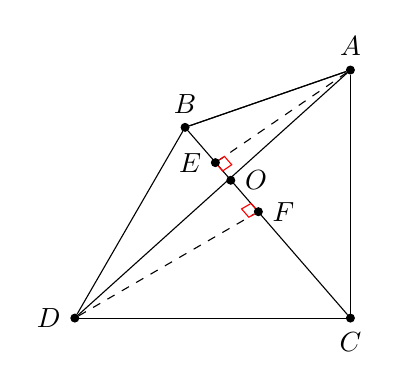
\begin{tikzpicture}
[scale = 0.7,>=stealth,point/.style = {draw, circle, fill = black, inner sep = 1pt}]
\node (A) at (5,4.5)[point,label=above :$A$] {};
\node (D) at (0,0)[point,label=left :$D$] {};
\node (C) at (5,0)[point,label=below :$C$] {};
\node (B) at (2,3.46)[point,label=above :$B$] {};
\node (E) at (2.55,2.82)[point,label=left :$E$] {};
\node (F) at (3.33,1.93)[point,label=right :$F$] {};
\node (O) at (2.83,2.50)[point,label=right :$O$] {};
\draw (D)--(C);
\draw (D)--(A);
\draw (A)--(B);
\draw (C)--(A);
\draw (A)--(B);
\draw (B)--(D);
\draw (B)--(C);
\draw [dashed] (A) -- (E);
\draw [dashed] (D) -- (F);
\tkzMarkRightAngle[draw=red,size=.2](A,E,C)
\tkzMarkRightAngle[draw=red,size=.2](D,F,E)
\end{tikzpicture}
\end{figure}
\end{frame}
\begin{frame}

\begin{itemize}
\item DC=a=4  CA=b=6
\item D=(0,0) \\
\item C=(4,0)\\
\item O=$\frac{(A+D)}{2}$ \\
\item B=(2O$-$C)=B(2.05,5.63)\\
\item A(p,q)\\
\item p=$\frac{a^2+c^2-b^2}{2a}$ q=$\sqrt{c^2-p^2}$\\
\item A(6.05,5.63)\\
\item F=(3.57,1.23)\\
\item E=(2.47,4.40)
\end{itemize}

\end{frame}
\begin{frame}
\begin{figure}
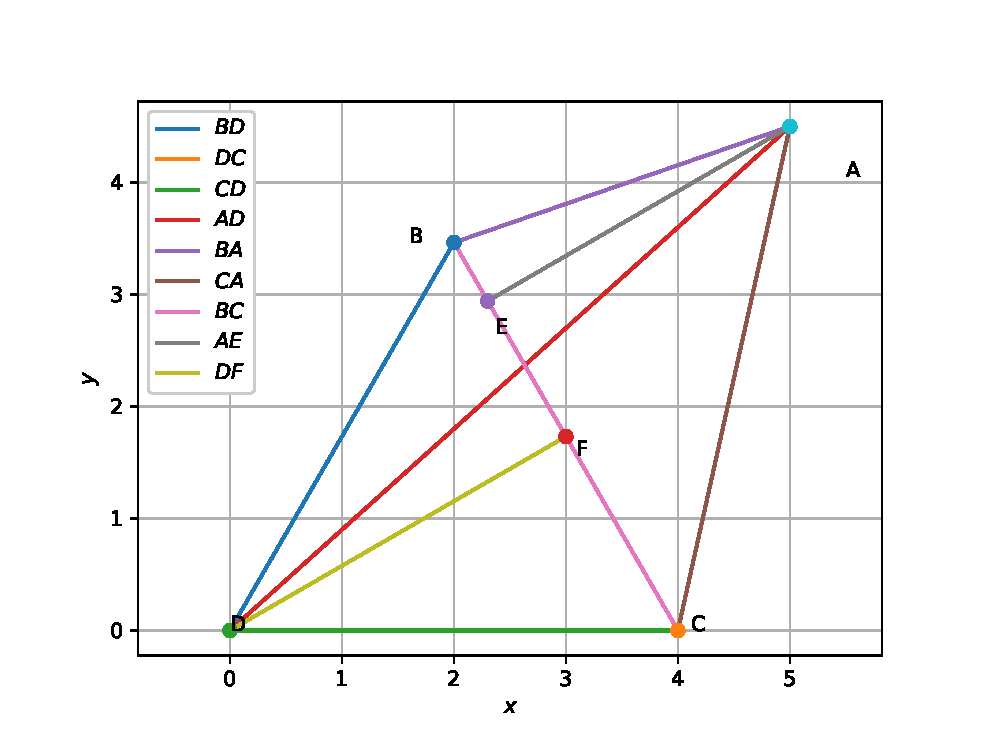
\includegraphics[scale=0.4]{./figs/triexe.eps}
\end{figure}
\url{https://github.com/Rajolep/_Geometry/blob/master/codes/triangle/triangexer.py}
\end{frame}
\begin{frame}
\begin{align*}
AE\perp BC , DF\perp BC\\
Area of \triangle{ABC} = \frac{1}{2}(BC)(AE)\\
Area of \triangle{DBC} = \frac{1}{2}(BC)(DF)\\
\frac{ar\triangle{ABC}}{ar\triangle{DBC}}=\frac{\frac{1}{2}(BC)(AE)}{\frac{1}{2}(BC)(DF)}\\  
\frac{ar\triangle{ABC}}{ar\triangle{DBC}}=\frac{AE}{DF}\\
\frac{AE}{DF}=\frac{AO}{DO}\\
\angle{AEO}=\angle{DFO}..... RA\\
\angle{AEO}=\angle{DOF}..... VOA\\
\triangle{AOE} \sim \triangle{DOF}\\
\frac{AE}{DF}=\frac{AO}{DO}\\
\end{align*}
\end{frame}
\begin{frame}
\begin{align*}
AE=2.407\\
BC=e=9.10294\\
DF=3.4756\\
AO=AE...(1)\\
DO=DF...(2)\\
\end{align*}
From  (1) and  (2)\\
Area of $\triangle{ABC} = \frac{1}{2}(BC)(AE)  = 38.0739$\\
Area of$ \triangle{DBC} = \frac{1}{2}(BC)(DF)  = 38.0739$\\
\end{frame}
\begin{frame}
\frametitle{Problem Statement-Triangle Construction}
\begin{enumerate}[label=(\roman*)]
\item Construct $\triangle LMN$ right angled at M such that LN $=$ 5  MN $=$ 3\\

\textbf{Soln:}\\
\url{https://github.com/Rajolep/_Geometry/blob/master/codes/triangle/draw_triangle.py}
\url{https://github.com/Rajolep/_Geometry/blob/master/figs/construc.tex}
\begin{figure}
\begin{tikzpicture}
[scale =0.7,>=stealth,point/.style = {draw, circle, fill = black, inner sep = 1pt},]
\node (L) at (0,4)[point,label=above :$L$] {};
\node (M) at (0,0)[point,label=below :$M$] {};
\node (N) at (3,0)[point,label=below :$N$] {};

\draw (L)--(M);
\draw (M)--(N);
\draw (L)--(N);

\tkzMarkRightAngle[draw=red,size=.2](L,M,N)
 
\end{tikzpicture}
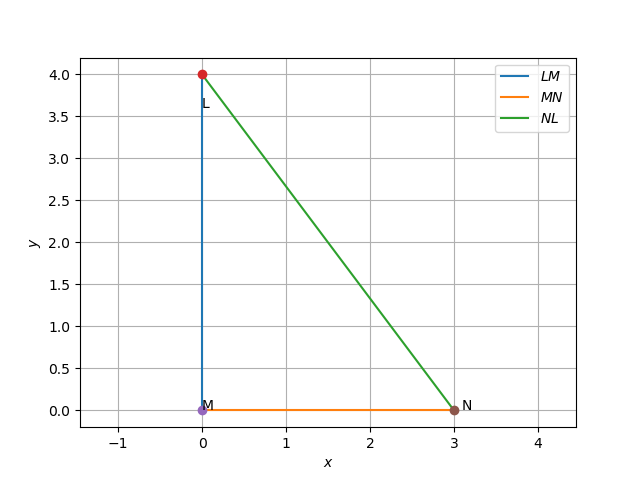
\includegraphics[scale=0.2]{./figs/tricon.png}
\end{figure}
\end{enumerate}
\end{frame}
\begin{frame}
\frametitle{Problem Statement-Miscellenous}
\begin{enumerate}[label=(\roman*)]
\item In a circular table cover of radius 32 cm, a design is formed leaving an equilateral $\triangle{ABC}$
in the middle. Find the area of the design.\\
\end{enumerate}
\textbf{Soln:}\\
  Given: R=32cm\\
\url{https://github.com/Rajolep/_Geometry/blob/master/codes/miscel.py}
\begin{figure}
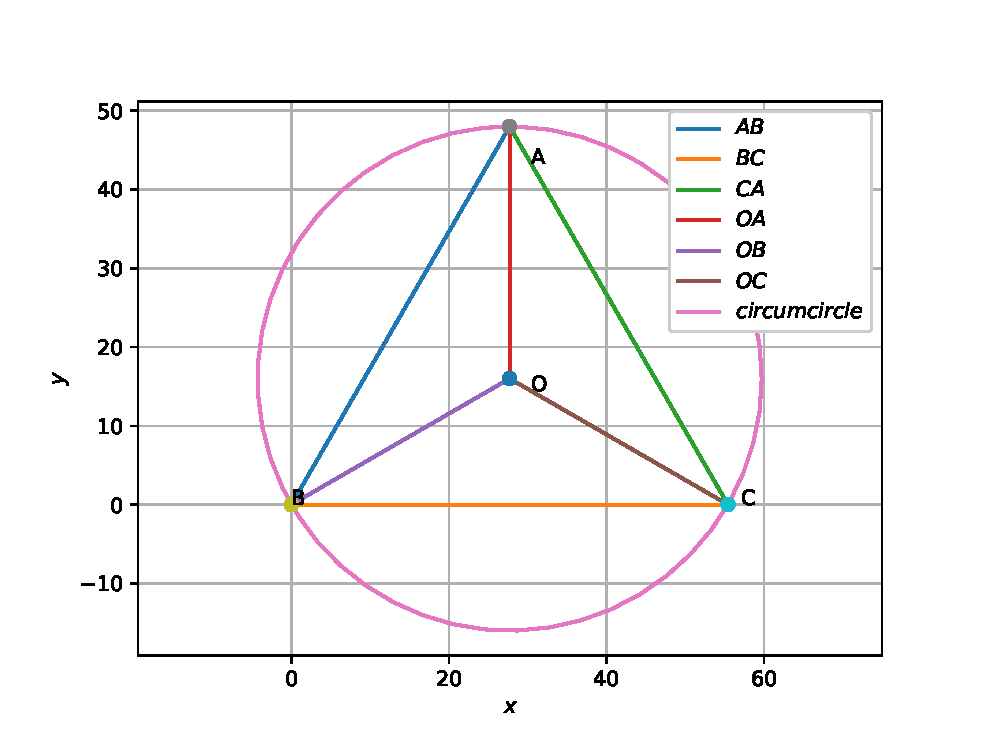
\includegraphics[scale=0.3]{./figs/misc.eps}
\end{figure}
\end{frame}
\begin{frame}
\url{https://github.com/Rajolep/_Geometry/blob/master/figs/miscell.tex}
\begin{figure}
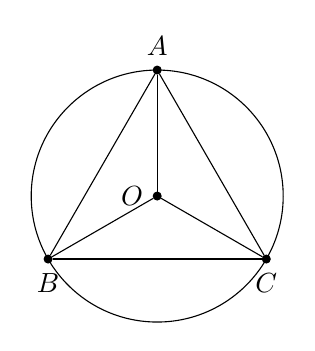
\begin{tikzpicture}
[scale =0.05,>=stealth,point/.style = {draw, circle, fill = black, inner sep = 1pt},]
\def\rad{32}
\coordinate [point, label={left: $O$ }] (O) at (27.712,16);
\draw (O) circle (\rad);
\node (B) at (0,0)[point,label=below :$B$] {};
\node (C) at (55.42,0)[point,label=below :$C$] {};
\node (A) at (27.712,48)[point,label=above :$A$] {};
\draw (A)--(C);
\draw (O)--(C);
\draw (O)--(B);
\draw (A)--(O);
\draw (A)--(B);
\draw (B)--(C);

\end{tikzpicture}

\end{figure}
%\begin{align*}
%\triangle{BOC} = 120\degree \\
%BO=OC=32\\
%BC=\sqrt{(BO)^2+(OC)^2-2(BO)(OC)\cos(120)}=55.425\\
%a=\sqrt{(2R)^2-2(R)^2)\cos{120}}\\
%s=\frac{a+b+c}{2}\\
%\end{{align*}
%Area of design = $\pi(R)(R)$ - $\sqrt{s(s-a)(s-b)(s-c)}$\\
%Area = 1886.81
\end{frame}
\begin{frame}
\frametitle{Problem Statement-Quadrilateral Construction}
\begin{enumerate}[label=(\roman*)]
\item Construct DEAR with DE = 4, EA = 5, AR = 4.5, $\angle {E}$ = 60$\degree$ and $\angle {A}$ = 90$\degree$.\\
\textbf{Soln:}\\
given:-  DE = 4, EA = 5, AR = 4.5, $\angle {E}$ = 60$\degree$ and $\angle {A}$ = 90$\degree$\\
\url{https://github.com/Rajolep/_Geometry/blob/master/codes/Quad/drawquad.py}
\url{https://github.com/Rajolep/_Geometry/blob/master/figs/quadccon.tex}
\begin{figure}
\begin{tikzpicture}
[scale =0.9,>=stealth,point/.style = {draw, circle, fill = black, inner sep = 1pt},]
\node (D) at (2,3.464)[point,label=above :$D$] {};
\node (E) at (0,0)[point,label=below :$E$] {};
\node (A) at (5,0)[point,label=below :$A$] {};
\node (R) at (5,4.5)[point,label=above :$R$] {};
\draw (D)--(E);
\draw (E)--(A);
\draw (A)--(R);
\draw (R)--(D);
\tkzMarkAngle[fill=white!60,size=.3](A,E,D)
\tkzLabelAngle[pos=0.65](A,E,D){$60$}
\tkzMarkRightAngle[draw=black,size=.2](R,A,E)
\end{tikzpicture}

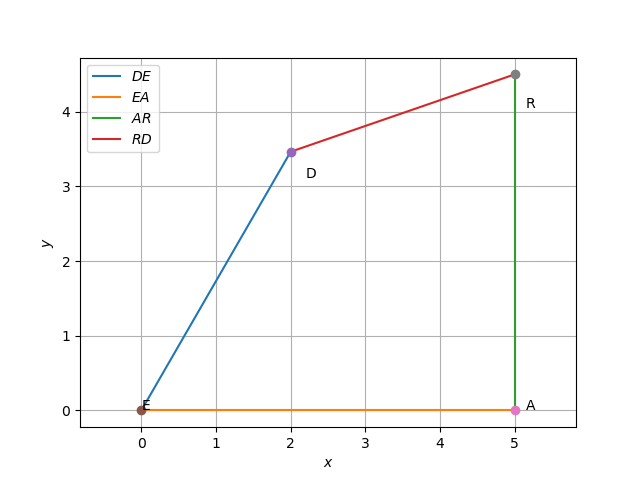
\includegraphics[scale=0.2]{./figs/quadcon.png}
\end{figure}
  \end{enumerate}

\end{frame}

\end{document}